\section{Results}
\label{sec:results}

\begin{table}[t]
\centering
\caption{Main result: \prauc{} on the stratified evaluation subsample (single seed). Columns are the
GBDT baseline and the three adaptation strategies of the \emph{same} pretrained backbone. $\Delta$ is
the gain of the third attention over standard fine-tuning. \textbf{Bold} marks the best adaptation
arm; \textsuperscript{$\ast$} marks where it also beats the GBDT.}
\label{tab:main}
\small
\begin{tabular}{lcccc c}
\toprule
Dataset & GBDT & probe & fine-tune & \makecell{fine-tune\\$+$ cross-attn} & $\Delta$ \\
\midrule
Synthetic (control) & $0.849$ & $0.793$ & $\mathbf{0.829}$ & $0.823$ & $-0.006$ \\
TalkingData         & $0.405$ & $0.486$ & $0.678$ & $\mathbf{0.714}^{\ast}$ & $+0.036$ \\
IEEE-CIS            & $0.294$ & $0.163$ & $0.167$ & $\mathbf{0.230}$ & $+0.063$ \\
Retailrocket        & $0.630$ & $0.344$ & $0.467$ & $\mathbf{0.534}$ & $+0.067$ \\
\bottomrule
\end{tabular}
\end{table}

% Count/pattern duality figure (pgfplots). Numeric x + manual ticklabels so
% explicit y-error tuples (+- (0,std)) parse cleanly (symbolic x coords do not).
\begin{figure}[t]
\centering
\begin{subfigure}{0.49\linewidth}\centering
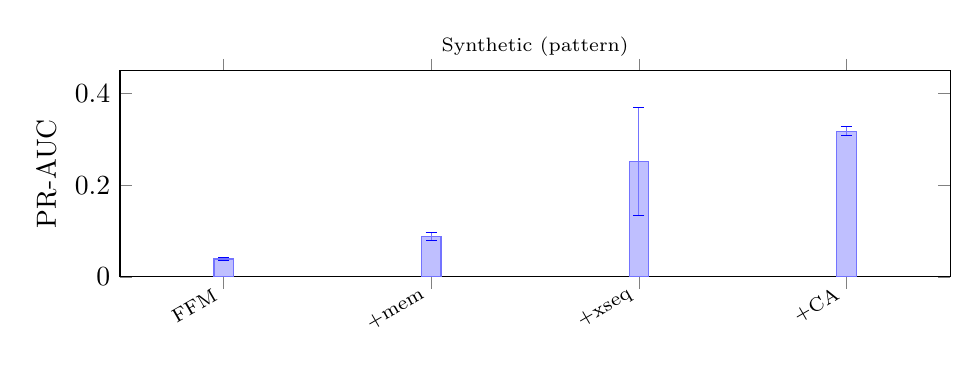
\begin{tikzpicture}
\begin{axis}[width=\linewidth, height=4.2cm, ybar, bar width=7pt,
  ymin=0, ymax=0.45, ylabel={PR-AUC}, ylabel near ticks,
  xmin=0.5, xmax=4.5, xtick={1,2,3,4},
  xticklabels={FFM,+mem,+xseq,+CA}, x tick label style={rotate=30,anchor=east,font=\scriptsize},
  title={\scriptsize Synthetic (pattern)}, title style={yshift=-1ex}]
\addplot+[fill=blue!25, draw=blue!55, error bars/.cd, y dir=both, y explicit] coordinates {
  (1,0.039) +- (0,0.004) (2,0.088) +- (0,0.009)
  (3,0.252) +- (0,0.117) (4,0.318) +- (0,0.010)};
\end{axis}
\end{tikzpicture}
\end{subfigure}\hfill
\begin{subfigure}{0.49\linewidth}\centering
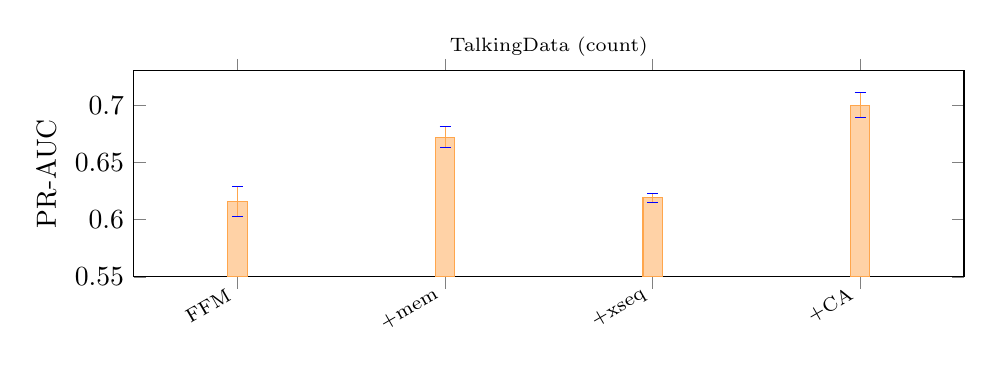
\begin{tikzpicture}
\begin{axis}[width=\linewidth, height=4.2cm, ybar, bar width=7pt,
  ymin=0.55, ymax=0.73, ylabel={PR-AUC}, ylabel near ticks,
  xmin=0.5, xmax=4.5, xtick={1,2,3,4},
  xticklabels={FFM,+mem,+xseq,+CA}, x tick label style={rotate=30,anchor=east,font=\scriptsize},
  title={\scriptsize TalkingData (count)}, title style={yshift=-1ex}]
\addplot+[fill=orange!35, draw=orange!70, error bars/.cd, y dir=both, y explicit] coordinates {
  (1,0.616) +- (0,0.013) (2,0.672) +- (0,0.009)
  (3,0.619) +- (0,0.004) (4,0.700) +- (0,0.011)};
\end{axis}
\end{tikzpicture}
\end{subfigure}
\caption{Count vs.\ pattern, and the unifying fix (PR-AUC, mean\,$\pm$\,std, 3 seeds).
\textbf{Left (synthetic, pattern signal):} raw-neighbour attention (\texttt{+xseq}) has a high mean
but is wildly seed-unstable; the count-aware encoder (\texttt{+CA}) is stable and highest.
\textbf{Right (TalkingData, count signal):} \texttt{+xseq} alone barely moves over the per-account
FFM (a bounded window truncates a velocity magnitude), the memory (count) path helps, and
\texttt{+CA} wins. One module (\texttt{+CA}) is best in both regimes. Note the different $y$-ranges.}
\label{fig:results}
\end{figure}


Table~\ref{tab:main} and Figure~\ref{fig:results} report the full result. Three findings.

\paragraph{The third attention gives a consistent relational gain.} On all three datasets that
contain a cross-account signal, adding cross-sequence attention improves \prauc{} over standard
fine-tuning of the same backbone --- \num{+0.036} on TalkingData, \num{+0.063} on IEEE-CIS, and
\num{+0.067} on Retailrocket. The ordering probe $\to$ fine-tune $\to$ fine-tune$+$cross-attention is
monotonic in every case: unfreezing the backbone helps, and the third attention helps further.

\paragraph{The gain is the relational signal, not added capacity.} On the synthetic control --- where
the fraud is per-account by construction and no relational signal exists at the shared entity --- the
\emph{same} added module yields no gain (\num{-0.006}; fine-tune \num{0.829} vs.\ cross-attention
\num{0.823}). Identical extra parameters that lift the three relational datasets do nothing here.
This isolates the improvement as cross-sequence information rather than model capacity, and doubles
as a specificity check: the module does not spuriously inflate a task it should not help.

\paragraph{It can beat a strong GBDT, and generalises beyond fraud.} On TalkingData the fine-tuned
FFM with the third attention reaches \num{0.714}, clearing the strong GBDT baseline (\num{0.405}):
here the FFM models a user's own click sequence, a signal the tree lacks, and the third attention
adds the cross-user IP signal on top. On IEEE-CIS and Retailrocket the FFM trails the GBDT
(\num{0.230} vs.\ \num{0.294}; \num{0.534} vs.\ \num{0.630}) --- there the relational signal is close
to a scalar velocity that a tree exploits efficiently (\S\ref{sec:discussion}) --- yet the third
attention still delivers its relational lift. Notably Retailrocket is a \emph{non-fraud} conversion
task: the same module, unchanged, recovers the ``item trending now'' signal, showing the approach is
not fraud-specific.
